\documentclass[12pt,twoside]{report}
\usepackage[utf8]{inputenc}
\usepackage{graphicx}
\graphicspath{ {images/} }
\usepackage{indentfirst}
\usepackage[a4paper,width=150mm,top=25mm,bottom=25mm,bindingoffset=6mm]{geometry}
\usepackage{fancyhdr}
\pagestyle{fancy}
\fancyhead{}
\fancyhead[RO,LE]{Domain Decomposition as a Method to Solve the Poisson Problem}
\fancyfoot{}
\fancyfoot[LE,RO]{\thepage}
\fancyfoot[LO,CE]{Chapter \thechapter}
\fancyfoot[CO,RE]{Brenton Peck}
\renewcommand{\headrulewidth}{0.4pt}
\renewcommand{\footrulewidth}{0.4pt}
\usepackage{caption}
\usepackage[backend=bibtex8]{biblatex}
\addbibresource{chapters/references.bib}
\usepackage{amsmath}
\usepackage{tikz, subfigure}
\usetikzlibrary{arrows}
\tikzstyle{every node}=[draw,shape=circle]
\usepackage{mathtools}
\usepackage{listings}

\begin{document}

\begin{titlepage}
    \begin{center}
        \vspace*{1cm}
        
	\Huge
        \textbf{Domain Decomposition as a Finite Difference Method to Solve Applications of the Poisson Problem}
        
        \vspace{0.5cm}
	\LARGE
        Additive Shwarz
        
        \vspace{1.5cm}
        
        \textbf{Brenton Peck}
        
        \vfill
        
        A thesis presented for the degree of\\
        Bachelor of Science in Applied Mathematics
        
        \vspace{0.8cm}
        
        
\includegraphics[width=0.4\textwidth]{university}
        
	\Large
        Department of Mathematics\\
        Boise State University\\
        United States of America\\
        \today
        
    \end{center}
\end{titlepage}

\chapter*{Acknowledgments}
This thesis would not have been possible without the support of Dr. Donna Calhoun and Scott Aiton who have answered my seemingly innumerous questions with grace. I am especially indebted to my adviser Dr. Grady Wright who has been incredibly supportive of my research and who has constantly given advice and direction in both my academics as-well-as my career goals.

I am grateful to everyone with whom I have have had the pleasure of working with while researching and writing this thesis. Each professor that I have interacted with in the math department at Boise State University has provided me with extensive personal and professional guidance as I finish my degree and begin life as both a graduate and first-time father.

During my time as a student, no one has been more important to me than my family. I would like to thank my parents for their constant love, support, and understanding. Most importantly, I wish to thank my wife, Teri, for her unending love and support and for understanding the amount of time that goes into doing research and completing a degree.

\tableofcontents

\chapter{Introduction}
In high performance computing, one often deals with very large matrices that would be exorbitantly expensive to compute using direct solvers. One method of handling these matrices is to decompose them into smaller matrices that can then be approximated iteratively and in parallel. This method is known as domain decomposition. There are two ways of decomposing a domain into smaller sub-domains, overlapping and non-overlapping as-well-as two methods of evaluating these, node-centered and cell-centered. For this paper we will assume Dirichlet-Dirichlet boundary conditions.

In the first method, we will first use the node centered method and split the domain into smaller sub-domains that overlap each other such that the values at the boundaries between the sub-domains are equivalent. This method leaves the sub-domains coupled at the boundary and each of the sub-domains must communicate values to its adjacent sub-domains. There is some parallelism that is achieved using this method in a staggered fashion; however, the more sub-domains we decompose to, the more wait time there is for the sub-domains furthest from the first sub-domain to be approximated due to each sub-domain having to wait to start being approximated until receiving boundary values from the previous sub-domain. We can parallelize this method further by not communicating values between the sub-domains, but rather making an initial guess at the boundary value and then iterating until a Neumann boundary condition on the interior boundaries has been satisfied to within a given tolerance. This allows all of the sub-domains to be approximated simultaneously instead of in a staggered fashion.

The second method decouples the sub-domains entirely allowing us to achieve full parallelism in solving the sub-domains. This is done by dividing the domain into sub-domains such that they share the boundary or boundaries without overlapping. If we solve for the values on the boundaries, then we can turn the single Dirichlet-Dirichlet boundary problem into an arbitrary number of smaller Dirichlet-Dirichlet problems. These boundary values can be found by solving the Schur-complement system.

\chapter{Motivations and Background}
I will be examining the application of domain decomposition methods specifically applied to the Poisson problem which is a type of elliptic problem particularly important to the realm of physics. The Poisson equation $\nabla^2u = f$ involves the Laplacian and a function that only depends on its space variables \cite{Farlow}. This allows us to use a central-difference approximation for a given system. 

While there are many applications of the Poisson problem, in my research we are approximating it to model pressure as part of the over-arching goal of modeling wind through mountainous regions. Attempting to model weather without any surface interactions is a challenging problem by itself. When we begin to introduce more complex geography, the problem becomes much more complex. These large problems result in very large matrices which we would like to avoid computing using direct solvers. By decomposing these rather large problems into smaller de-coupled problems, we can achieve massive parallelization that enables us to approximate the original system in a comparably small amount of time.

A further method, which I will not discuss in detail, we utilize in my research to reduce the size of the problem is called adaptive mesh refinement. This is motivated by fluid dynamics, where the frictional force causes the highest rate of change in pressure to occur at boundaries where the fluid interacts with another object. In our situation, this means the the pressure is going to change the most where the wind interacts with the mountain. This means that we can gain a fairly accurate approximation of the pressure at points away from the surface of the mountain using significantly larger interval widths which make for much smaller problems. As we approach the surface of the mountain, however, we need much smaller interval widths to achieve the same level of accuracy. This can be done by starting with a courser mesh size as needed away from the mountain and further sub-dividing up portions of that mesh until we have a fine enough mesh to approximate the problem at the boundary of the mountainside.

\chapter{Iterative Methods}
The most natural place to start, although not the easiest to motivate, is the 1-dimensional problem. I will show that the equations using a second-order central-difference approximation along a 1-dimensional domain interface ensure that the values at the boundary of two nodes are equivalent. Subsequently, I will demonstrate that this extends naturally to 2-dimensional problems.

We start by analyzing figure \ref{fig:1dgrid} which depicts a line and decomposing it into two sub-domains in the subsequent figure \ref{fig:1dgriddecomp}. Nodes $u_0$ and $u_8$ are ghost nodes used to solve along the line from $u_1$ to $u_7$. Each node can be approximated using the central-difference approximation

\begin{equation}
	u''(x_{j}) \cong \frac{1}{h^2}[u_{j-1} - 2u_{j} + u_{j+1}]
\end{equation} 

\begin {figure}[htbp]
  \centering
    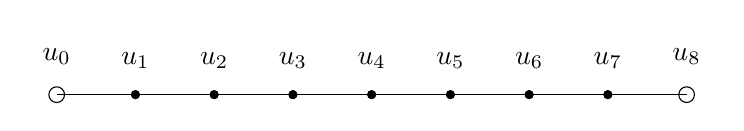
\begin{tikzpicture}
\tikzset{every node}=[draw,shape=circle]

\draw (0,0) node[circle,inner sep=2pt,label=above:$u_0$](a){} -- (1,0) 
node[circle,fill,inner sep=1pt,label=above:$u_1$](b){};
\draw (1,0) node[circle,fill,inner sep=1pt](a){} -- (2,0) 
node[circle,fill,inner sep=1pt,label=above:$u_2$](b){};
\draw (2,0) node[circle,fill,inner sep=1pt](a){} -- (3,0) 
node[circle,fill,inner sep=1pt,label=above:$u_3$](b){};
\draw (3,0) node[circle,fill,inner sep=1pt](a){} -- (4,0) 
node[circle,fill,inner sep=1pt,label=above:$u_4$](b){};
\draw (4,0) node[circle,fill,inner sep=1pt](a){} -- (5,0) 
node[circle,fill,inner sep=1pt,label=above:$u_5$](b){};
\draw (5,0) node[circle,fill,inner sep=1pt](a){} -- (6,0) 
node[circle,fill,inner sep=1pt,label=above:$u_6$](b){};
\draw (6,0) node[circle,fill,inner sep=1pt](a){} -- (7,0) 
node[circle,fill,inner sep=1pt,label=above:$u_7$](b){};
\draw (7,0) node[circle,fill,inner sep=1pt](a){} -- (8,0) 
node[circle,inner sep=2pt,label=above:$u_8$](b){};

   \end{tikzpicture}
     \caption{1-D line before domain decomposition. \label{fig:1dgrid}}
  \end{figure}

In figure \ref{fig:1dgriddecomp}, the domain has been decomposed into two parts, $\Omega_0$ and $\Omega_1$, that share the boundary $u_4^0 = u_0^1$. Each of the sub-domains then have two ghost nodes such that on the first iteration $u_5^0$ is set to an initial guess and on each subsequent iteration $u_{-1}^1$ receives its value from $u_3^0$ and $u_5^0$ receives its value from $u_1^1$.
\begin {figure}[htbp]
  \centering
    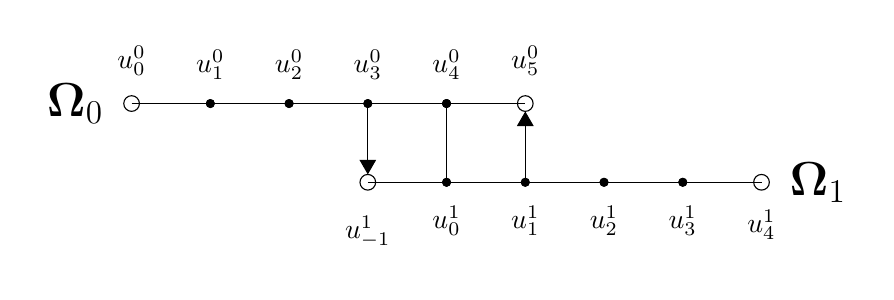
\begin{tikzpicture}[>=triangle 60]
\tikzset{every node}=[draw,shape=circle]

\draw (0,0) node[circle,inner sep=2pt,label=above:$u_0^0$,label=left:\LARGE$\boldsymbol\Omega_0$](a){} -- (1,0) 
node[circle,fill,inner sep=1pt,label=above:$u_1^0$](b){};
\draw (1,0) node[circle,fill,inner sep=1pt](a){} -- (2,0) 
node[circle,fill,inner sep=1pt,label=above:$u_2^0$](b){};
\draw (2,0) node[circle,fill,inner sep=1pt](a){} -- (3,0) 
node[circle,fill,inner sep=1pt,label=above:$u_3^0$](b){};
\draw (3,0) node[circle,fill,inner sep=1pt](a){} -- (4,0) 
node[circle,fill,inner sep=1pt,label=above:$u_4^0$](b){};
\draw (4,0) node[circle,fill,inner sep=1pt](a){} -- (5,0) 
node[circle,inner sep=2pt,label=above:$u_5^0$](b){};

\draw[->] (3,0) -- (3,-0.9);
\draw (4,0) node[circle,fill,inner sep=1pt](a){} -- (4,-1);
\draw[->] (5,-1) -- (5,-0.1);

\draw[yshift=-1cm] (3,0) node[circle,inner sep=2pt,label=below:$u_{-1}^1$](a){} -- (4,0) 
node[circle,fill,inner sep=1pt,label=below:$u_{0}^1$](b){};
\draw[yshift=-1cm] (4,0) node[circle,fill,inner sep=1pt](a){} -- (5,0) 
node[circle,fill,inner sep=1pt,label=below:$u_{1}^1$](b){};
\draw[yshift=-1cm] (5,0) node[circle,fill,inner sep=1pt](a){} -- (6,0) 
node[circle,fill,inner sep=1pt,label=below:$u_{2}^1$](b){};
\draw[yshift=-1cm] (6,0) node[circle,fill,inner sep=1pt](a){} -- (7,0) 
node[circle,fill,inner sep=1pt,label=below:$u_{3}^1$](b){};
\draw[yshift=-1cm] (7,0) node[circle,fill,inner sep=1pt](a){} -- (8,0) 
node[circle,inner sep=2pt,label=below:$u_{4}^1$,label=right:\LARGE$\boldsymbol\Omega_1$](b){};


   \end{tikzpicture}
     \caption{1-D line after domain decomposition. \label{fig:1dgriddecomp}}
  \end{figure}

This decomposition leads to the following equations on the boundary when solving the Poisson problem where $f$ is the exact solution at each point.
\begin{alignat*}{4}
u_3^0 & {}-{} &  2u_4^0 & {}+{} & u_5^0 & {}={} & f_4^0 \\
u_{-1}^1 & {}-{} &  2u_0^1 & {}+{} & u_1^1 & {}={} & f_0^1
\end{alignat*}

From these equations we know that $f_4^0 = f_1^1$ and since at each iteration $u_{-1}^1$ receives its value from $u_3^0$ and $u_5^0$ receives its value from $u_1^1$ we see that the equations become $u_3^0 - 2u_4^0 + u_1^1 = f_4^0 = u_3^0 - 2u_0^1 + u_1^1$ and thus $u_4^0 = u_0^1$.

Now we will attempt the 2-D case. We start by making a box and decomposing it into two sub-domains as seen in the subsequent figures. I have adopted the notation of $u_{xy}$ where x is the x-coordinate and y is the y-coordinate. Nodes along $x = 0$ and $4$ as-well-as nodes along $y = 0$ and $8$ are ghost nodes. We can approximate each node using the central-difference approximation

\begin{equation}
	u''(x_{j}) \cong \frac{1}{h^2}[u_{i-1,j} + u_{i+1,j} - 4u_{i,j} + u_{i,j-1} + u_{i,j+1}]
\end{equation}

\begin {figure}[htbp]
  \centering
    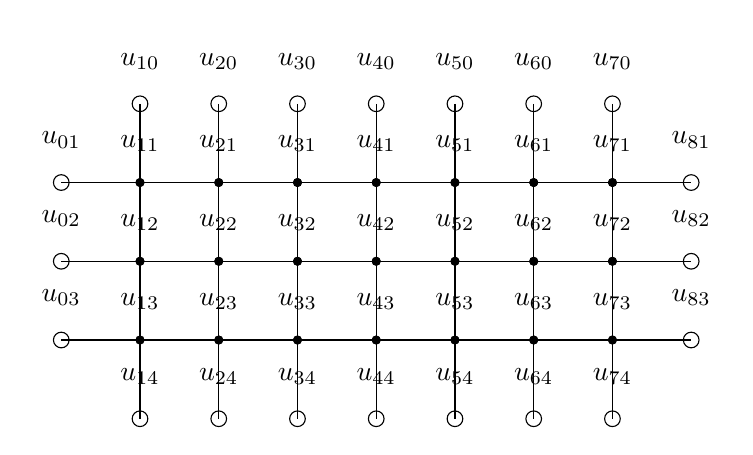
\begin{tikzpicture}
\tikzset{every node}=[draw,shape=circle]

\draw (1,0) node[circle,inner sep=2pt,label=above:$u_{10}$](b){} -- (1,-4);
\draw (2,0) node[circle,inner sep=2pt,label=above:$u_{20}$](b){} -- (2,-4);
\draw (3,0) node[circle,inner sep=2pt,label=above:$u_{30}$](b){} -- (3,-4);
\draw (4,0) node[circle,inner sep=2pt,label=above:$u_{40}$](b){} -- (4,-4);
\draw (5,0) node[circle,inner sep=2pt,label=above:$u_{50}$](b){} -- (5,-4);
\draw (6,0) node[circle,inner sep=2pt,label=above:$u_{60}$](b){} -- (6,-4);
\draw (7,0) node[circle,inner sep=2pt,label=above:$u_{70}$](b){} -- (7,-4);

\draw (0,-1) node[circle,inner sep=2pt,label=above:$u_{01}$](a){} -- (1,-1) 
node[circle,fill,inner sep=1pt,label=above:$u_{11}$](b){};
\draw (1,-1) node[circle,fill,inner sep=1pt](a){} -- (2,-1) 
node[circle,fill,inner sep=1pt,label=above:$u_{21}$](b){};
\draw (2,-1) node[circle,fill,inner sep=1pt](a){} -- (3,-1) 
node[circle,fill,inner sep=1pt,label=above:$u_{31}$](b){};
\draw (3,-1) node[circle,fill,inner sep=1pt](a){} -- (4,-1) 
node[circle,fill,inner sep=1pt,label=above:$u_{41}$](b){};
\draw (4,-1) node[circle,fill,inner sep=1pt](a){} -- (5,-1) 
node[circle,fill,inner sep=1pt,label=above:$u_{51}$](b){};
\draw (5,-1) node[circle,fill,inner sep=1pt](a){} -- (6,-1) 
node[circle,fill,inner sep=1pt,label=above:$u_{61}$](b){};
\draw (6,-1) node[circle,fill,inner sep=1pt](a){} -- (7,-1) 
node[circle,fill,inner sep=1pt,label=above:$u_{71}$](b){};
\draw (7,-1) node[circle,fill,inner sep=1pt](a){} -- (8,-1) 
node[circle,inner sep=2pt,label=above:$u_{81}$](b){};

\draw (0,-2) node[circle,inner sep=2pt,label=above:$u_{02}$](a){} -- (1,-2) 
node[circle,fill,inner sep=1pt,label=above:$u_{12}$](b){};
\draw (1,-2) node[circle,fill,inner sep=1pt](a){} -- (2,-2) 
node[circle,fill,inner sep=1pt,label=above:$u_{22}$](b){};
\draw (2,-2) node[circle,fill,inner sep=1pt](a){} -- (3,-2) 
node[circle,fill,inner sep=1pt,label=above:$u_{32}$](b){};
\draw (3,-2) node[circle,fill,inner sep=1pt](a){} -- (4,-2) 
node[circle,fill,inner sep=1pt,label=above:$u_{42}$](b){};
\draw (4,-2) node[circle,fill,inner sep=1pt](a){} -- (5,-2) 
node[circle,fill,inner sep=1pt,label=above:$u_{52}$](b){};
\draw (5,-2) node[circle,fill,inner sep=1pt](a){} -- (6,-2) 
node[circle,fill,inner sep=1pt,label=above:$u_{62}$](b){};
\draw (6,-2) node[circle,fill,inner sep=1pt](a){} -- (7,-2) 
node[circle,fill,inner sep=1pt,label=above:$u_{72}$](b){};
\draw (7,-2) node[circle,fill,inner sep=1pt](a){} -- (8,-2) 
node[circle,inner sep=2pt,label=above:$u_{82}$](b){};

\draw (0,-3) node[circle,inner sep=2pt,label=above:$u_{03}$](a){} -- (1,-3) 
node[circle,fill,inner sep=1pt,label=above:$u_{13}$](b){};
\draw (1,-3) node[circle,fill,inner sep=1pt](a){} -- (2,-3) 
node[circle,fill,inner sep=1pt,label=above:$u_{23}$](b){};
\draw (2,-3) node[circle,fill,inner sep=1pt](a){} -- (3,-3) 
node[circle,fill,inner sep=1pt,label=above:$u_{33}$](b){};
\draw (3,-3) node[circle,fill,inner sep=1pt](a){} -- (4,-3) 
node[circle,fill,inner sep=1pt,label=above:$u_{43}$](b){};
\draw (4,-3) node[circle,fill,inner sep=1pt](a){} -- (5,-3) 
node[circle,fill,inner sep=1pt,label=above:$u_{53}$](b){};
\draw (5,-3) node[circle,fill,inner sep=1pt](a){} -- (6,-3) 
node[circle,fill,inner sep=1pt,label=above:$u_{63}$](b){};
\draw (6,-3) node[circle,fill,inner sep=1pt](a){} -- (7,-3) 
node[circle,fill,inner sep=1pt,label=above:$u_{73}$](b){};
\draw (7,-3) node[circle,fill,inner sep=1pt](a){} -- (8,-3) 
node[circle,inner sep=2pt,label=above:$u_{83}$](b){};

\draw (1,-4) node[circle,inner sep=2pt,label=above:$u_{14}$](b){};
\draw (2,-4) node[circle,inner sep=2pt,label=above:$u_{24}$](b){};
\draw (3,-4) node[circle,inner sep=2pt,label=above:$u_{34}$](b){};
\draw (4,-4) node[circle,inner sep=2pt,label=above:$u_{44}$](b){};
\draw (5,-4) node[circle,inner sep=2pt,label=above:$u_{54}$](b){};
\draw (6,-4) node[circle,inner sep=2pt,label=above:$u_{64}$](b){};
\draw (7,-4) node[circle,inner sep=2pt,label=above:$u_{74}$](b){};

   \end{tikzpicture}
     \caption{2-D box before domain decomposition. \label{fig:2dgrid1}}
  \end{figure}

Similar to the 1-D case, the domain has been decomposed into two parts, $\Omega_0$ and $\Omega_1$, that share the boundary $u_{4y}^0 = u_{0y}^1$. Each of the sub-domains then have ghost nodes such that for each j, $u_{-1,j}^1$ receives its value from $u_{3,j}^0$ and $u_{5,j}^0$ receives its value from $u_{1,j}^1$ every iteration.
\begin {figure}[htbp]
  \centering
    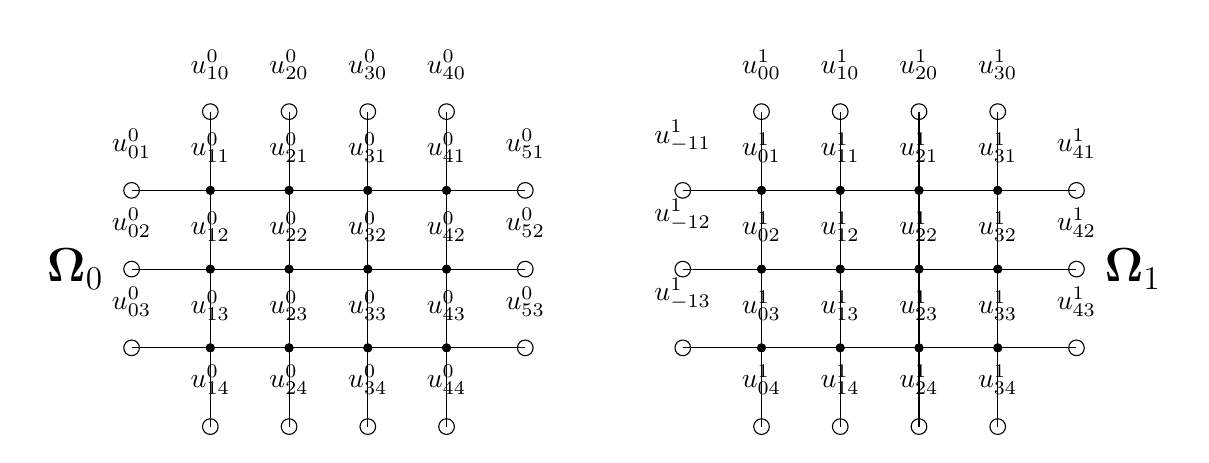
\begin{tikzpicture}
\tikzset{every node}=[draw,shape=circle]

\draw (1,0) node[circle,inner sep=2pt,label=above:$u_{10}^0$](b){} -- (1,-4);
\draw (2,0) node[circle,inner sep=2pt,label=above:$u_{20}^0$](b){} -- (2,-4);
\draw (3,0) node[circle,inner sep=2pt,label=above:$u_{30}^0$](b){} -- (3,-4);
\draw (4,0) node[circle,inner sep=2pt,label=above:$u_{40}^0$](b){} -- (4,-4);

\draw (8,0) node[circle,inner sep=2pt,label=above:$u_{00}^1$](b){} -- (8,-4);
\draw (9,0) node[circle,inner sep=2pt,label=above:$u_{10}^1$](b){} -- (9,-4);
\draw (10,0) node[circle,inner sep=2pt,label=above:$u_{20}^1$](b){} -- (10,-4);
\draw (11,0) node[circle,inner sep=2pt,label=above:$u_{30}^1$](b){} -- (11,-4);

\draw (0,-1) node[circle,inner sep=2pt,label=above:$u_{01}^0$](a){} -- (1,-1) 
node[circle,fill,inner sep=1pt,label=above:$u_{11}^0$](b){};
\draw (1,-1) node[circle,fill,inner sep=1pt](a){} -- (2,-1) 
node[circle,fill,inner sep=1pt,label=above:$u_{21}^0$](b){};
\draw (2,-1) node[circle,fill,inner sep=1pt](a){} -- (3,-1) 
node[circle,fill,inner sep=1pt,label=above:$u_{31}^0$](b){};
\draw (3,-1) node[circle,fill,inner sep=1pt](a){} -- (4,-1) 
node[circle,fill,inner sep=1pt,label=above:$u_{41}^0$](b){};
\draw (4,-1) node[circle,fill,inner sep=1pt](a){} -- (5,-1) 
node[circle,inner sep=2pt,label=above:$u_{51}^0$](b){};

\draw (7,-1) node[circle,inner sep=2pt,label=above:$u_{-11}^1$](a){} -- (8,-1) 
node[circle,fill,inner sep=1pt,label=above:$u_{01}^1$](b){};
\draw (8,-1) node[circle,fill,inner sep=1pt](a){} -- (9,-1) 
node[circle,fill,inner sep=1pt,label=above:$u_{11}^1$](b){};
\draw (9,-1) node[circle,fill,inner sep=1pt](a){} -- (10,-1) 
node[circle,fill,inner sep=1pt,label=above:$u_{21}^1$](b){};
\draw (10,-1) node[circle,fill,inner sep=1pt](a){} -- (11,-1) 
node[circle,fill,inner sep=1pt,label=above:$u_{31}^1$](b){};
\draw (11,-1) node[circle,fill,inner sep=1pt](a){} -- (12,-1) 
node[circle,inner sep=2pt,label=above:$u_{41}^1$](b){};

\draw (0,-2) node[circle,inner sep=2pt,label=above:$u_{02}^0$,label=left:\LARGE$\boldsymbol\Omega_0$](a){} -- (1,-2) 
node[circle,fill,inner sep=1pt,label=above:$u_{12}^0$](b){};
\draw (1,-2) node[circle,fill,inner sep=1pt](a){} -- (2,-2) 
node[circle,fill,inner sep=1pt,label=above:$u_{22}^0$](b){};
\draw (2,-2) node[circle,fill,inner sep=1pt](a){} -- (3,-2) 
node[circle,fill,inner sep=1pt,label=above:$u_{32}^0$](b){};
\draw (3,-2) node[circle,fill,inner sep=1pt](a){} -- (4,-2) 
node[circle,fill,inner sep=1pt,label=above:$u_{42}^0$](b){};
\draw (4,-2) node[circle,fill,inner sep=1pt](a){} -- (5,-2) 
node[circle,inner sep=2pt,label=above:$u_{52}^0$](b){};

\draw (7,-2) node[circle,inner sep=2pt,label=above:$u_{-12}^1$](a){} -- (8,-2) 
node[circle,fill,inner sep=1pt,label=above:$u_{02}^1$](b){};
\draw (8,-2) node[circle,fill,inner sep=1pt](a){} -- (9,-2) 
node[circle,fill,inner sep=1pt,label=above:$u_{12}^1$](b){};
\draw (9,-2) node[circle,fill,inner sep=1pt](a){} -- (10,-2) 
node[circle,fill,inner sep=1pt,label=above:$u_{22}^1$](b){};
\draw (10,-2) node[circle,fill,inner sep=1pt](a){} -- (11,-2) 
node[circle,fill,inner sep=1pt,label=above:$u_{32}^1$](b){};
\draw (11,-2) node[circle,fill,inner sep=1pt](a){} -- (12,-2) 
node[circle,inner sep=2pt,label=above:$u_{42}^1$,label=right:\LARGE$\boldsymbol\Omega_1$](b){};

\draw (0,-3) node[circle,inner sep=2pt,label=above:$u_{03}^0$](a){} -- (1,-3) 
node[circle,fill,inner sep=1pt,label=above:$u_{13}^0$](b){};
\draw (1,-3) node[circle,fill,inner sep=1pt](a){} -- (2,-3) 
node[circle,fill,inner sep=1pt,label=above:$u_{23}^0$](b){};
\draw (2,-3) node[circle,fill,inner sep=1pt](a){} -- (3,-3) 
node[circle,fill,inner sep=1pt,label=above:$u_{33}^0$](b){};
\draw (3,-3) node[circle,fill,inner sep=1pt](a){} -- (4,-3) 
node[circle,fill,inner sep=1pt,label=above:$u_{43}^0$](b){};
\draw (4,-3) node[circle,fill,inner sep=1pt](a){} -- (5,-3) 
node[circle,inner sep=2pt,label=above:$u_{53}^0$](b){};

\draw (7,-3) node[circle,inner sep=2pt,label=above:$u_{-13}^1$](a){} -- (8,-3) 
node[circle,fill,inner sep=1pt,label=above:$u_{03}^1$](b){};
\draw (8,-3) node[circle,fill,inner sep=1pt](a){} -- (9,-3) 
node[circle,fill,inner sep=1pt,label=above:$u_{13}^1$](b){};
\draw (9,-3) node[circle,fill,inner sep=1pt](a){} -- (10,-3) 
node[circle,fill,inner sep=1pt,label=above:$u_{23}^1$](b){};
\draw (10,-3) node[circle,fill,inner sep=1pt](a){} -- (11,-3) 
node[circle,fill,inner sep=1pt,label=above:$u_{33}^1$](b){};
\draw (11,-3) node[circle,fill,inner sep=1pt](a){} -- (12,-3) 
node[circle,inner sep=2pt,label=above:$u_{43}^1$](b){};

\draw (1,-4) node[circle,inner sep=2pt,label=above:$u_{14}^0$](b){};
\draw (2,-4) node[circle,inner sep=2pt,label=above:$u_{24}^0$](b){};
\draw (3,-4) node[circle,inner sep=2pt,label=above:$u_{34}^0$](b){};
\draw (4,-4) node[circle,inner sep=2pt,label=above:$u_{44}^0$](b){};

\draw (8,-4) node[circle,inner sep=2pt,label=above:$u_{04}^1$](b){};
\draw (9,-4) node[circle,inner sep=2pt,label=above:$u_{14}^1$](b){};
\draw (10,-4) node[circle,inner sep=2pt,label=above:$u_{24}^1$](b){};
\draw (11,-4) node[circle,inner sep=2pt,label=above:$u_{34}^1$](b){};

   \end{tikzpicture}
     \caption{2-D box after domain decomposition. \label{fig:2dgriddecomp1}}
  \end{figure}

\pagebreak
The resulting decomposition yields the following equations on the boundary for the Poisson problem.
\begin{alignat*}{6}
u_{31}^0 & {}+{} & u_{51}^0 & {}+{} & u_{40}^0 & {}+{} &  u_{42}^0 & {}-{} &  4u_{41}^0 & {}={} & f_{41}^0 \\
u_{-11}^1 & {}+{} & u_{11}^1 & {}+{} & u_{00}^1 & {}+{} &  u_{02}^1 & {}-{} &  4u_{01}^1 & {}={} & f_{01}^1\\
u_{32}^0 & {}+{} & u_{52}^0 & {}+{} & u_{41}^0 & {}+{} &  u_{43}^0 & {}-{} &  4u_{42}^0 & {}={} & f_{42}^0 \\
u_{-12}^1 & {}+{} & u_{12}^1 & {}+{} & u_{01}^1 & {}+{} &  u_{03}^1 & {}-{} &  4u_{02}^1 & {}={} & f_{02}^1\\
u_{33}^0 & {}+{} & u_{53}^0 & {}+{} & u_{42}^0 & {}+{} &  u_{44}^0 & {}-{} &  4u_{43}^0 & {}={} & f_{43}^0 \\
u_{-13}^1 & {}+{} & u_{13}^1 & {}+{} & u_{02}^1 & {}+{} &  u_{04}^1 & {}-{} &  4u_{03}^1 & {}={} & f_{03}^1
\end{alignat*}

From these equations we know that for each j, $f_{4,j}^0 = f_{0,j}^1$ and since at each iteration $u_{-1,j}^1$ receives its value from $u_{3,j}^0$ and $u_{5,j}^0$ receives its value from $u_{1,j}^1$ we see that after reducing, the equations become:
\begin{alignat*}{11}
u_{40}^0 & {}+{} &  u_{42}^0 & {}-{} &  4u_{41}^0 & {}={} & u_{00}^1 & {}+{} &  u_{02}^1 & {}-{} &  4u_{01}^1\\
u_{41}^0 & {}+{} &  u_{43}^0 & {}-{} &  4u_{42}^0 & {}={} & u_{01}^1 & {}+{} &  u_{03}^1 & {}-{} &  4u_{02}^1\\
u_{42}^0 & {}+{} &  u_{44}^0 & {}-{} &  4u_{43}^0 & {}={} & u_{02}^1 & {}+{} &  u_{04}^1 & {}-{} &  4u_{03}^1
\end{alignat*}

Furthermore, since we have boundary conditions, the ghost nodes on the boundary are known to be equivalent. That is, $u_{40}^0 = u_{00}^1$ and $u_{44}^0 = u_{04}^1$ which gives the following system of equations.
\begin{alignat}{6}
\label{eq:3.3} && u_{42}^0 & {}-{} &  4u_{41}^0 & {}={} & u_{02}^1 & {}-{} &  4u_{01}^1 && \\
\label{eq:3.4}u_{41}^0 & {}+{} &  u_{43}^0 & {}-{} &  4u_{42}^0 & {}={} & u_{01}^1 & {}+{} &  u_{03}^1 & {}-{} &  4u_{02}^1\\
\label{eq:3.5}&& u_{42}^0 & {}+{} &  4u_{43}^0 & {}={} & u_{02}^1 & {}+{} &  4u_{03}^1 &&
\end{alignat}

Now if we both solve \ref{eq:3.3} and \ref{eq:3.5} for $u_{02}^1$ and $u_{42}^0$ and plug into \ref{eq:3.4}, as-well-as subtract \ref{eq:3.5} from \ref{eq:3.3} we get
\begin{alignat*}{4} 
	u_{41}^0 & {}+{} &  u_{43}^0 & {}={} & u_{01}^1 & {}+{} &  u_{03}^1\\
	-u_{41}^0 & {}+{} &  u_{43}^0 & {}={} & -u_{01}^1 & {}+{} &  u_{03}^1
\end{alignat*}

Adding and subtracting these equations together and then plugging into \ref{eq:3.4} we arrive at the final result we are looking for. 
\begin{alignat*}{2} 
	u_{41}^0 & {}={} & u_{01}^1\\
	u_{42}^0 & {}={} & u_{02}^1\\
	u_{43}^0 & {}={} & u_{03}^1
\end{alignat*}

For the sake of thoroughness, we will extend this to 4 sub-domains as shown in the next two figures. Similar to our proof that the boundary values between $\Omega_0$ and $\Omega_1$ are equivalent, it can be shown that the boundary values between $\Omega_0$ and $\Omega_2$ are equivalent as are those between $\Omega_1$ and $\Omega_3$. What remains then is to show that the boundary value shared by all 4 nodes is equivalent for each; that is, $u_{43}^0 = u_{03}^1 = u_{40}^2 = u_{00}^3$.
\begin {figure}[htbp]
  \centering
    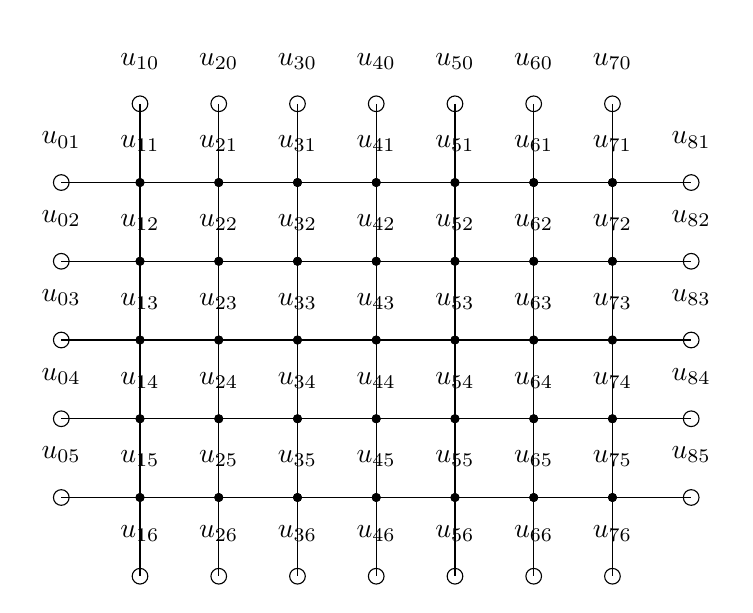
\begin{tikzpicture}
\tikzset{every node}=[draw,shape=circle]

\draw (1,0) node[circle,inner sep=2pt,label=above:$u_{10}$](b){} -- (1,-6)
	node[circle,inner sep=2pt,label=above:$u_{16}$](b){};
\draw (2,0) node[circle,inner sep=2pt,label=above:$u_{20}$](b){} -- (2,-6)
	node[circle,inner sep=2pt,label=above:$u_{26}$](b){};
\draw (3,0) node[circle,inner sep=2pt,label=above:$u_{30}$](b){} -- (3,-6)
	node[circle,inner sep=2pt,label=above:$u_{36}$](b){};
\draw (4,0) node[circle,inner sep=2pt,label=above:$u_{40}$](b){} -- (4,-6)
	node[circle,inner sep=2pt,label=above:$u_{46}$](b){};
\draw (5,0) node[circle,inner sep=2pt,label=above:$u_{50}$](b){} -- (5,-6)
	node[circle,inner sep=2pt,label=above:$u_{56}$](b){};
\draw (6,0) node[circle,inner sep=2pt,label=above:$u_{60}$](b){} -- (6,-6)
	node[circle,inner sep=2pt,label=above:$u_{66}$](b){};
\draw (7,0) node[circle,inner sep=2pt,label=above:$u_{70}$](b){} -- (7,-6)
	node[circle,inner sep=2pt,label=above:$u_{76}$](b){};

\draw (0,-1) node[circle,inner sep=2pt,label=above:$u_{01}$](a){} -- (1,-1) 
node[circle,fill,inner sep=1pt,label=above:$u_{11}$](b){};
\draw (1,-1) node[circle,fill,inner sep=1pt](a){} -- (2,-1) 
node[circle,fill,inner sep=1pt,label=above:$u_{21}$](b){};
\draw (2,-1) node[circle,fill,inner sep=1pt](a){} -- (3,-1) 
node[circle,fill,inner sep=1pt,label=above:$u_{31}$](b){};
\draw (3,-1) node[circle,fill,inner sep=1pt](a){} -- (4,-1) 
node[circle,fill,inner sep=1pt,label=above:$u_{41}$](b){};
\draw (4,-1) node[circle,fill,inner sep=1pt](a){} -- (5,-1) 
node[circle,fill,inner sep=1pt,label=above:$u_{51}$](b){};
\draw (5,-1) node[circle,fill,inner sep=1pt](a){} -- (6,-1) 
node[circle,fill,inner sep=1pt,label=above:$u_{61}$](b){};
\draw (6,-1) node[circle,fill,inner sep=1pt](a){} -- (7,-1) 
node[circle,fill,inner sep=1pt,label=above:$u_{71}$](b){};
\draw (7,-1) node[circle,fill,inner sep=1pt](a){} -- (8,-1) 
node[circle,inner sep=2pt,label=above:$u_{81}$](b){};

\draw (0,-2) node[circle,inner sep=2pt,label=above:$u_{02}$](a){} -- (1,-2) 
node[circle,fill,inner sep=1pt,label=above:$u_{12}$](b){};
\draw (1,-2) node[circle,fill,inner sep=1pt](a){} -- (2,-2) 
node[circle,fill,inner sep=1pt,label=above:$u_{22}$](b){};
\draw (2,-2) node[circle,fill,inner sep=1pt](a){} -- (3,-2) 
node[circle,fill,inner sep=1pt,label=above:$u_{32}$](b){};
\draw (3,-2) node[circle,fill,inner sep=1pt](a){} -- (4,-2) 
node[circle,fill,inner sep=1pt,label=above:$u_{42}$](b){};
\draw (4,-2) node[circle,fill,inner sep=1pt](a){} -- (5,-2) 
node[circle,fill,inner sep=1pt,label=above:$u_{52}$](b){};
\draw (5,-2) node[circle,fill,inner sep=1pt](a){} -- (6,-2) 
node[circle,fill,inner sep=1pt,label=above:$u_{62}$](b){};
\draw (6,-2) node[circle,fill,inner sep=1pt](a){} -- (7,-2) 
node[circle,fill,inner sep=1pt,label=above:$u_{72}$](b){};
\draw (7,-2) node[circle,fill,inner sep=1pt](a){} -- (8,-2) 
node[circle,inner sep=2pt,label=above:$u_{82}$](b){};

\draw (0,-3) node[circle,inner sep=2pt,label=above:$u_{03}$](a){} -- (1,-3) 
node[circle,fill,inner sep=1pt,label=above:$u_{13}$](b){};
\draw (1,-3) node[circle,fill,inner sep=1pt](a){} -- (2,-3) 
node[circle,fill,inner sep=1pt,label=above:$u_{23}$](b){};
\draw (2,-3) node[circle,fill,inner sep=1pt](a){} -- (3,-3) 
node[circle,fill,inner sep=1pt,label=above:$u_{33}$](b){};
\draw (3,-3) node[circle,fill,inner sep=1pt](a){} -- (4,-3) 
node[circle,fill,inner sep=1pt,label=above:$u_{43}$](b){};
\draw (4,-3) node[circle,fill,inner sep=1pt](a){} -- (5,-3) 
node[circle,fill,inner sep=1pt,label=above:$u_{53}$](b){};
\draw (5,-3) node[circle,fill,inner sep=1pt](a){} -- (6,-3) 
node[circle,fill,inner sep=1pt,label=above:$u_{63}$](b){};
\draw (6,-3) node[circle,fill,inner sep=1pt](a){} -- (7,-3) 
node[circle,fill,inner sep=1pt,label=above:$u_{73}$](b){};
\draw (7,-3) node[circle,fill,inner sep=1pt](a){} -- (8,-3) 
node[circle,inner sep=2pt,label=above:$u_{83}$](b){};

\draw (0,-4) node[circle,inner sep=2pt,label=above:$u_{04}$](a){} -- (1,-4) 
node[circle,fill,inner sep=1pt,label=above:$u_{14}$](b){};
\draw (1,-4) node[circle,fill,inner sep=1pt](a){} -- (2,-4) 
node[circle,fill,inner sep=1pt,label=above:$u_{24}$](b){};
\draw (2,-4) node[circle,fill,inner sep=1pt](a){} -- (3,-4) 
node[circle,fill,inner sep=1pt,label=above:$u_{34}$](b){};
\draw (3,-4) node[circle,fill,inner sep=1pt](a){} -- (4,-4) 
node[circle,fill,inner sep=1pt,label=above:$u_{44}$](b){};
\draw (4,-4) node[circle,fill,inner sep=1pt](a){} -- (5,-4) 
node[circle,fill,inner sep=1pt,label=above:$u_{54}$](b){};
\draw (5,-4) node[circle,fill,inner sep=1pt](a){} -- (6,-4) 
node[circle,fill,inner sep=1pt,label=above:$u_{64}$](b){};
\draw (6,-4) node[circle,fill,inner sep=1pt](a){} -- (7,-4) 
node[circle,fill,inner sep=1pt,label=above:$u_{74}$](b){};
\draw (7,-4) node[circle,fill,inner sep=1pt](a){} -- (8,-4) 
node[circle,inner sep=2pt,label=above:$u_{84}$](b){};

\draw (0,-5) node[circle,inner sep=2pt,label=above:$u_{05}$](a){} -- (1,-5) 
node[circle,fill,inner sep=1pt,label=above:$u_{15}$](b){};
\draw (1,-5) node[circle,fill,inner sep=1pt](a){} -- (2,-5) 
node[circle,fill,inner sep=1pt,label=above:$u_{25}$](b){};
\draw (2,-5) node[circle,fill,inner sep=1pt](a){} -- (3,-5) 
node[circle,fill,inner sep=1pt,label=above:$u_{35}$](b){};
\draw (3,-5) node[circle,fill,inner sep=1pt](a){} -- (4,-5) 
node[circle,fill,inner sep=1pt,label=above:$u_{45}$](b){};
\draw (4,-5) node[circle,fill,inner sep=1pt](a){} -- (5,-5) 
node[circle,fill,inner sep=1pt,label=above:$u_{55}$](b){};
\draw (5,-5) node[circle,fill,inner sep=1pt](a){} -- (6,-5) 
node[circle,fill,inner sep=1pt,label=above:$u_{65}$](b){};
\draw (6,-5) node[circle,fill,inner sep=1pt](a){} -- (7,-5) 
node[circle,fill,inner sep=1pt,label=above:$u_{75}$](b){};
\draw (7,-5) node[circle,fill,inner sep=1pt](a){} -- (8,-5) 
node[circle,inner sep=2pt,label=above:$u_{85}$](b){};


   \end{tikzpicture}
     \caption{2-D box before domain decomposition. \label{fig:2dgrid2}}
  \end{figure}
\begin {figure}[htbp]
  \centering
    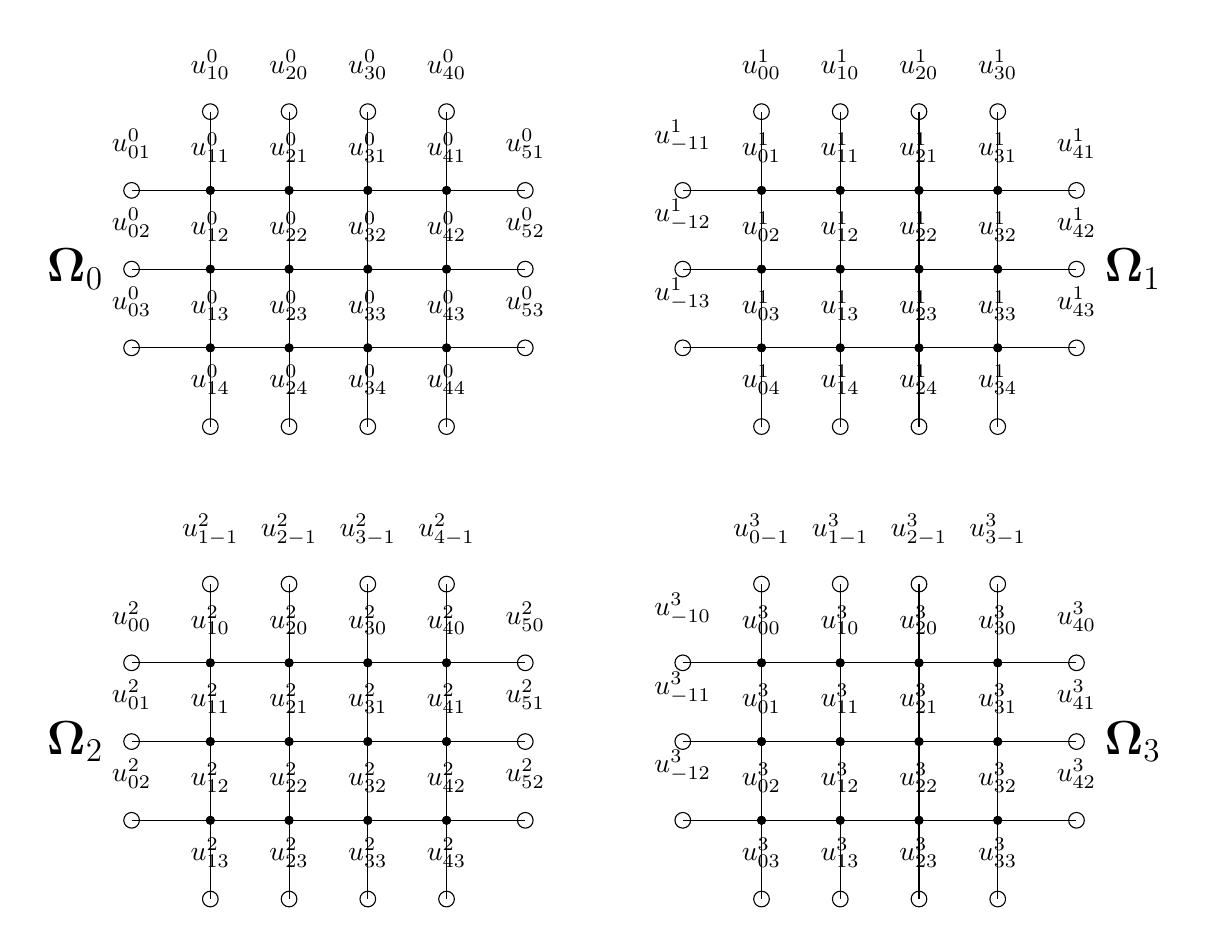
\begin{tikzpicture}
\tikzset{every node}=[draw,shape=circle]

%% Verticle Lines
%% Omega 0
\draw (1,0) node[circle,inner sep=2pt,label=above:$u_{10}^0$](b){} -- (1,-4)
	node[circle,inner sep=2pt,label=above:$u_{14}^0$](b){};
\draw (2,0) node[circle,inner sep=2pt,label=above:$u_{20}^0$](b){} -- (2,-4)
	node[circle,inner sep=2pt,label=above:$u_{24}^0$](b){};
\draw (3,0) node[circle,inner sep=2pt,label=above:$u_{30}^0$](b){} -- (3,-4)
	node[circle,inner sep=2pt,label=above:$u_{34}^0$](b){};
\draw (4,0) node[circle,inner sep=2pt,label=above:$u_{40}^0$](b){} -- (4,-4)
	node[circle,inner sep=2pt,label=above:$u_{44}^0$](b){};
%% Omega 1
\draw (8,0) node[circle,inner sep=2pt,label=above:$u_{00}^1$](b){} -- (8,-4)
	node[circle,inner sep=2pt,label=above:$u_{04}^1$](b){};
\draw (9,0) node[circle,inner sep=2pt,label=above:$u_{10}^1$](b){} -- (9,-4)
	node[circle,inner sep=2pt,label=above:$u_{14}^1$](b){};
\draw (10,0) node[circle,inner sep=2pt,label=above:$u_{20}^1$](b){} -- (10,-4)
	node[circle,inner sep=2pt,label=above:$u_{24}^1$](b){};
\draw (11,0) node[circle,inner sep=2pt,label=above:$u_{30}^1$](b){} -- (11,-4)
	node[circle,inner sep=2pt,label=above:$u_{34}^1$](b){};
%% Omega 2
\draw (1,-6) node[circle,inner sep=2pt,label=above:$u_{1-1}^2$](b){} -- (1,-10)
	node[circle,inner sep=2pt,label=above:$u_{13}^2$](b){};
\draw (2,-6) node[circle,inner sep=2pt,label=above:$u_{2-1}^2$](b){} -- (2,-10)
	node[circle,inner sep=2pt,label=above:$u_{23}^2$](b){};
\draw (3,-6) node[circle,inner sep=2pt,label=above:$u_{3-1}^2$](b){} -- (3,-10)
	node[circle,inner sep=2pt,label=above:$u_{33}^2$](b){};
\draw (4,-6) node[circle,inner sep=2pt,label=above:$u_{4-1}^2$](b){} -- (4,-10)
	node[circle,inner sep=2pt,label=above:$u_{43}^2$](b){};
%% Omega 3
\draw (8,-6) node[circle,inner sep=2pt,label=above:$u_{0-1}^3$](b){} -- (8,-10)
	node[circle,inner sep=2pt,label=above:$u_{03}^3$](b){};
\draw (9,-6) node[circle,inner sep=2pt,label=above:$u_{1-1}^3$](b){} -- (9,-10)
	node[circle,inner sep=2pt,label=above:$u_{13}^3$](b){};
\draw (10,-6) node[circle,inner sep=2pt,label=above:$u_{2-1}^3$](b){} -- (10,-10)
	node[circle,inner sep=2pt,label=above:$u_{23}^3$](b){};
\draw (11,-6) node[circle,inner sep=2pt,label=above:$u_{3-1}^3$](b){} -- (11,-10)
	node[circle,inner sep=2pt,label=above:$u_{33}^3$](b){};
	
%% Horizontal Lines
%% Omega 0
\draw (0,-1) node[circle,inner sep=2pt,label=above:$u_{01}^0$](a){} -- (1,-1) 
node[circle,fill,inner sep=1pt,label=above:$u_{11}^0$](b){};
\draw (1,-1) node[circle,fill,inner sep=1pt](a){} -- (2,-1) 
node[circle,fill,inner sep=1pt,label=above:$u_{21}^0$](b){};
\draw (2,-1) node[circle,fill,inner sep=1pt](a){} -- (3,-1) 
node[circle,fill,inner sep=1pt,label=above:$u_{31}^0$](b){};
\draw (3,-1) node[circle,fill,inner sep=1pt](a){} -- (4,-1) 
node[circle,fill,inner sep=1pt,label=above:$u_{41}^0$](b){};
\draw (4,-1) node[circle,fill,inner sep=1pt](a){} -- (5,-1) 
node[circle,inner sep=2pt,label=above:$u_{51}^0$](b){};

\draw (0,-2) node[circle,inner sep=2pt,label=above:$u_{02}^0$,label=left:\LARGE$\boldsymbol\Omega_0$](a){} -- (1,-2) 
node[circle,fill,inner sep=1pt,label=above:$u_{12}^0$](b){};
\draw (1,-2) node[circle,fill,inner sep=1pt](a){} -- (2,-2) 
node[circle,fill,inner sep=1pt,label=above:$u_{22}^0$](b){};
\draw (2,-2) node[circle,fill,inner sep=1pt](a){} -- (3,-2) 
node[circle,fill,inner sep=1pt,label=above:$u_{32}^0$](b){};
\draw (3,-2) node[circle,fill,inner sep=1pt](a){} -- (4,-2) 
node[circle,fill,inner sep=1pt,label=above:$u_{42}^0$](b){};
\draw (4,-2) node[circle,fill,inner sep=1pt](a){} -- (5,-2) 
node[circle,inner sep=2pt,label=above:$u_{52}^0$](b){};

\draw (0,-3) node[circle,inner sep=2pt,label=above:$u_{03}^0$](a){} -- (1,-3) 
node[circle,fill,inner sep=1pt,label=above:$u_{13}^0$](b){};
\draw (1,-3) node[circle,fill,inner sep=1pt](a){} -- (2,-3) 
node[circle,fill,inner sep=1pt,label=above:$u_{23}^0$](b){};
\draw (2,-3) node[circle,fill,inner sep=1pt](a){} -- (3,-3) 
node[circle,fill,inner sep=1pt,label=above:$u_{33}^0$](b){};
\draw (3,-3) node[circle,fill,inner sep=1pt](a){} -- (4,-3) 
node[circle,fill,inner sep=1pt,label=above:$u_{43}^0$](b){};
\draw (4,-3) node[circle,fill,inner sep=1pt](a){} -- (5,-3) 
node[circle,inner sep=2pt,label=above:$u_{53}^0$](b){};

%% Omega 1
\draw (7,-1) node[circle,inner sep=2pt,label=above:$u_{-11}^1$](a){} -- (8,-1) 
node[circle,fill,inner sep=1pt,label=above:$u_{01}^1$](b){};
\draw (8,-1) node[circle,fill,inner sep=1pt](a){} -- (9,-1) 
node[circle,fill,inner sep=1pt,label=above:$u_{11}^1$](b){};
\draw (9,-1) node[circle,fill,inner sep=1pt](a){} -- (10,-1) 
node[circle,fill,inner sep=1pt,label=above:$u_{21}^1$](b){};
\draw (10,-1) node[circle,fill,inner sep=1pt](a){} -- (11,-1) 
node[circle,fill,inner sep=1pt,label=above:$u_{31}^1$](b){};
\draw (11,-1) node[circle,fill,inner sep=1pt](a){} -- (12,-1) 
node[circle,inner sep=2pt,label=above:$u_{41}^1$](b){};

\draw (7,-2) node[circle,inner sep=2pt,label=above:$u_{-12}^1$](a){} -- (8,-2) 
node[circle,fill,inner sep=1pt,label=above:$u_{02}^1$](b){};
\draw (8,-2) node[circle,fill,inner sep=1pt](a){} -- (9,-2) 
node[circle,fill,inner sep=1pt,label=above:$u_{12}^1$](b){};
\draw (9,-2) node[circle,fill,inner sep=1pt](a){} -- (10,-2) 
node[circle,fill,inner sep=1pt,label=above:$u_{22}^1$](b){};
\draw (10,-2) node[circle,fill,inner sep=1pt](a){} -- (11,-2) 
node[circle,fill,inner sep=1pt,label=above:$u_{32}^1$](b){};
\draw (11,-2) node[circle,fill,inner sep=1pt](a){} -- (12,-2) 
node[circle,inner sep=2pt,label=above:$u_{42}^1$,label=right:\LARGE$\boldsymbol\Omega_1$](b){};

\draw (7,-3) node[circle,inner sep=2pt,label=above:$u_{-13}^1$](a){} -- (8,-3) 
node[circle,fill,inner sep=1pt,label=above:$u_{03}^1$](b){};
\draw (8,-3) node[circle,fill,inner sep=1pt](a){} -- (9,-3) 
node[circle,fill,inner sep=1pt,label=above:$u_{13}^1$](b){};
\draw (9,-3) node[circle,fill,inner sep=1pt](a){} -- (10,-3) 
node[circle,fill,inner sep=1pt,label=above:$u_{23}^1$](b){};
\draw (10,-3) node[circle,fill,inner sep=1pt](a){} -- (11,-3) 
node[circle,fill,inner sep=1pt,label=above:$u_{33}^1$](b){};
\draw (11,-3) node[circle,fill,inner sep=1pt](a){} -- (12,-3) 
node[circle,inner sep=2pt,label=above:$u_{43}^1$](b){};

%% Omega 2
\draw (0,-7) node[circle,inner sep=2pt,label=above:$u_{00}^2$](a){} -- (1,-7) 
node[circle,fill,inner sep=1pt,label=above:$u_{10}^2$](b){};
\draw (1,-7) node[circle,fill,inner sep=1pt](a){} -- (2,-7) 
node[circle,fill,inner sep=1pt,label=above:$u_{20}^2$](b){};
\draw (2,-7) node[circle,fill,inner sep=1pt](a){} -- (3,-7) 
node[circle,fill,inner sep=1pt,label=above:$u_{30}^2$](b){};
\draw (3,-7) node[circle,fill,inner sep=1pt](a){} -- (4,-7) 
node[circle,fill,inner sep=1pt,label=above:$u_{40}^2$](b){};
\draw (4,-7) node[circle,fill,inner sep=1pt](a){} -- (5,-7) 
node[circle,inner sep=2pt,label=above:$u_{50}^2$](b){};

\draw (0,-8) node[circle,inner sep=2pt,label=above:$u_{01}^2$,label=left:\LARGE$\boldsymbol\Omega_2$](a){} -- (1,-8) 
node[circle,fill,inner sep=1pt,label=above:$u_{11}^2$](b){};
\draw (1,-8) node[circle,fill,inner sep=1pt](a){} -- (2,-8) 
node[circle,fill,inner sep=1pt,label=above:$u_{21}^2$](b){};
\draw (2,-8) node[circle,fill,inner sep=1pt](a){} -- (3,-8) 
node[circle,fill,inner sep=1pt,label=above:$u_{31}^2$](b){};
\draw (3,-8) node[circle,fill,inner sep=1pt](a){} -- (4,-8) 
node[circle,fill,inner sep=1pt,label=above:$u_{41}^2$](b){};
\draw (4,-8) node[circle,fill,inner sep=1pt](a){} -- (5,-8) 
node[circle,inner sep=2pt,label=above:$u_{51}^2$](b){};

\draw (0,-9) node[circle,inner sep=2pt,label=above:$u_{02}^2$](a){} -- (1,-9) 
node[circle,fill,inner sep=1pt,label=above:$u_{12}^2$](b){};
\draw (1,-9) node[circle,fill,inner sep=1pt](a){} -- (2,-9) 
node[circle,fill,inner sep=1pt,label=above:$u_{22}^2$](b){};
\draw (2,-9) node[circle,fill,inner sep=1pt](a){} -- (3,-9) 
node[circle,fill,inner sep=1pt,label=above:$u_{32}^2$](b){};
\draw (3,-9) node[circle,fill,inner sep=1pt](a){} -- (4,-9) 
node[circle,fill,inner sep=1pt,label=above:$u_{42}^2$](b){};
\draw (4,-9) node[circle,fill,inner sep=1pt](a){} -- (5,-9) 
node[circle,inner sep=2pt,label=above:$u_{52}^2$](b){};

%% Omega 3
\draw (7,-7) node[circle,inner sep=2pt,label=above:$u_{-10}^3$](a){} -- (8,-7) 
node[circle,fill,inner sep=1pt,label=above:$u_{00}^3$](b){};
\draw (8,-7) node[circle,fill,inner sep=1pt](a){} -- (9,-7) 
node[circle,fill,inner sep=1pt,label=above:$u_{10}^3$](b){};
\draw (9,-7) node[circle,fill,inner sep=1pt](a){} -- (10,-7) 
node[circle,fill,inner sep=1pt,label=above:$u_{20}^3$](b){};
\draw (10,-7) node[circle,fill,inner sep=1pt](a){} -- (11,-7) 
node[circle,fill,inner sep=1pt,label=above:$u_{30}^3$](b){};
\draw (11,-7) node[circle,fill,inner sep=1pt](a){} -- (12,-7) 
node[circle,inner sep=2pt,label=above:$u_{40}^3$](b){};

\draw (7,-8) node[circle,inner sep=2pt,label=above:$u_{-11}^3$](a){} -- (8,-8) 
node[circle,fill,inner sep=1pt,label=above:$u_{01}^3$](b){};
\draw (8,-8) node[circle,fill,inner sep=1pt](a){} -- (9,-8) 
node[circle,fill,inner sep=1pt,label=above:$u_{11}^3$](b){};
\draw (9,-8) node[circle,fill,inner sep=1pt](a){} -- (10,-8) 
node[circle,fill,inner sep=1pt,label=above:$u_{21}^3$](b){};
\draw (10,-8) node[circle,fill,inner sep=1pt](a){} -- (11,-8) 
node[circle,fill,inner sep=1pt,label=above:$u_{31}^3$](b){};
\draw (11,-8) node[circle,fill,inner sep=1pt](a){} -- (12,-8) 
node[circle,inner sep=2pt,label=above:$u_{41}^3$,label=right:\LARGE$\boldsymbol\Omega_3$](b){};

\draw (7,-9) node[circle,inner sep=2pt,label=above:$u_{-12}^3$](a){} -- (8,-9) 
node[circle,fill,inner sep=1pt,label=above:$u_{02}^3$](b){};
\draw (8,-9) node[circle,fill,inner sep=1pt](a){} -- (9,-9) 
node[circle,fill,inner sep=1pt,label=above:$u_{12}^3$](b){};
\draw (9,-9) node[circle,fill,inner sep=1pt](a){} -- (10,-9) 
node[circle,fill,inner sep=1pt,label=above:$u_{22}^3$](b){};
\draw (10,-9) node[circle,fill,inner sep=1pt](a){} -- (11,-9) 
node[circle,fill,inner sep=1pt,label=above:$u_{32}^3$](b){};
\draw (11,-9) node[circle,fill,inner sep=1pt](a){} -- (12,-9) 
node[circle,inner sep=2pt,label=above:$u_{42}^3$](b){};


   \end{tikzpicture}
     \caption{2-D box before domain decomposition. \label{fig:2dgriddecomp2}}
  \end{figure}

\pagebreak
Taking the values of the ghost nodes from their adjacent sub-domains and knowing that the function is equivalent on $f_{43}^0, f_{03}^1, f_{40}^2,$ and $f_{00}^3$, we obtain the following system of equations.
\begin{alignat*}{6} 
	& u_{42}^0 & {}+{} &  u_{41}^2 & {}+{} &  u_{33}^0 & {}+{} &  u_{13}^1 & {}-{} &  4u_{43}^0\\
	{}={} & u_{02}^1 & {}+{} &  u_{01}^3 & {}+{} &  u_{33}^0 & {}+{} &  u_{13}^1 & {}-{} &  4u_{03}^1\\
	{}={} & u_{42}^0 & {}+{} &  u_{41}^2 & {}+{} &  u_{30}^2 & {}+{} &  u_{10}^3 & {}-{} &  4u_{40}^2\\
	{}={} & u_{02}^1 & {}+{} &  u_{01}^3 & {}+{} &  u_{30}^2 & {}+{} &  u_{10}^3 & {}-{} &  4u_{00}^3
\end{alignat*}

Similarly, we know that ghost nodes sharing a boundary have the same value as shown below.
\begin{alignat*}{4} 
	u_{53}^0 & {}={} & u_{50}^2 & {}={} & u_{13}^1 & {}={} & u_{10}^3\\
	u_{44}^0 & {}={} & u_{04}^1 & {}={} & u_{41}^2 & {}={} & u_{01}^3\\
	u_{4-1}^2 & {}={} & u_{0-1}^3 & {}={} & u_{42}^0 & {}={} & u_{02}^1\\
	u_{-13}^1 & {}={} & u_{-10}^3 & {}={} & u_{33}^0 & {}={} & u_{30}^2
\end{alignat*}

Plugging these in, we get that $u_{43}^0 = u_{03}^1 = u_{40}^2 = u_{00}^3$ which is what we expected.







\chapter{Motivating Further Methods}
Using an overlapping domain method works well for some situations; however, there are situations that arise in which we would like to de-couple the sub-domains entirely. To motivate this method I will switch to a cell-centered approach. Starting in 1-D again we can visualize this using figure \ref{fig:4.1} which depicts a straight line with nodes at the center of each cell. We use the same central difference approximation we showed in equation \ref{eq:3.1}. The system boundaries are indicated at $u|_{x=0}$ and $u|_{x=1}$. For the non-overlapping case we define the boundary between two sub-domains as $\Gamma$. The value of $u$ on the boundary is then $\gamma$, so I have indicated the interior boundary $\Gamma$ at ${u|_{\Gamma} = \gamma}$.

\begin {figure}[htbp]
  \centering
    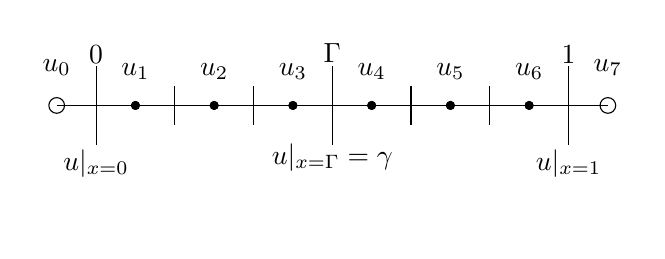
\begin{tikzpicture}
\tikzset{every node}=[draw,shape=circle]

\draw (0.5,0.5)  -- (0.5,-0.5);
\draw (0.5,0.2) node[draw=none,rectangle,label=above:$0$](a){};
\draw (0.5,0) node[draw=none,rectangle,label=below:$u|_{x=0}$](a){};
\draw (0,0) node[circle,inner sep=2pt,label=above:$u_0$](a){} -- (1,0) 
node[circle,fill,inner sep=1pt,label=above:$u_1$](b){};
\draw (1,0) node[circle,fill,inner sep=1pt](a){} -- (2,0) 
node[circle,fill,inner sep=1pt,label=above:$u_2$](b){};
\draw (1.5,0.25) -- (1.5,-0.25);
\draw (2,0) node[circle,fill,inner sep=1pt](a){} -- (3,0) 
node[circle,fill,inner sep=1pt,label=above:$u_3$](b){};
\draw (2.5,0.25) -- (2.5,-0.25);
\draw (3,0) node[circle,fill,inner sep=1pt](a){} -- (4,0) 
node[circle,fill,inner sep=1pt,label=above:$u_4$](b){};
\draw (3.5,0.5) -- (3.5,-0.5);
\draw (3.5,0.2) node[draw=none,rectangle,label=above:$\Gamma$](a){};
\draw (3.5,0.4) node[draw=none,rectangle,label=below:${u|_{x=\Gamma}=\gamma}$](a){};
\draw (4,0) node[circle,fill,inner sep=1pt](a){} -- (5,0) 
node[circle,fill,inner sep=1pt,label=above:$u_5$](b){};
\draw (4.5,0.25) -- (4.5,-0.25);
\draw (5,0) node[circle,fill,inner sep=1pt](a){} -- (6,0) 
node[circle,fill,inner sep=1pt,label=above:$u_6$](b){};
\draw (5.5,0.25) -- (5.5,-0.25);
\draw (6,0) node[circle,fill,inner sep=1pt](a){} -- (7,0) 
node[circle,inner sep=2pt,label=above:$u_7$](b){};
\draw (6.5,0.5) -- (6.5,-0.5);
\draw (6.5,0.2) node[draw=none,rectangle,label=above:$1$](a){};
\draw (6.5,0) node[draw=none,rectangle,label=below:$u|_{x=1}$](a){};

   \end{tikzpicture}
     \caption{1-D line before domain decomposition. \label{fig:4.1}}
  \end{figure}

We can define $\gamma$ to be the average of its neighbor nodes as shown in equation \ref{eq:4.1}.

\begin{equation}\label{eq:4.1}
	\gamma = \frac{u_{j} + u_{j+1}}{2}
\end{equation}

In figure \ref{fig:4.2} we have decomposed the domain into two sub-domains, $\Omega_0$ and $\Omega_1$. Unlike the node-centered case, the two sub-domains do not share any nodes or receive any values for ghost nodes. Instead we enforce equation \ref{eq:4.1} as a Dirichlet boundary condition between the two sub-domains. 

\pagebreak
\begin {figure}[htbp]
  \centering
    \begin{tikzpicture}[>=triangle 60]
\tikzset{every node}=[draw,shape=circle]

\draw (0.5,-0.5)  -- (0.5,0.5)
node[draw=none,rectangle,label=above:$u^0|_{x=0}$](a){};
\draw (0.5,-0.2) node[draw=none,rectangle,label=below:$0$](a){};
\draw (0,0) node[circle,inner sep=2pt,label=above:$u_0^0$,label=left:\LARGE$\boldsymbol\Omega_0$](a){} -- (1,0) 
node[circle,fill,inner sep=1pt,label=above:$u_1^0$](b){};
\draw (1,0) node[circle,fill,inner sep=1pt](a){} -- (2,0) 
node[circle,fill,inner sep=1pt,label=above:$u_2^0$](b){};
\draw (1.5,0.25) -- (1.5,-0.25);
\draw (2,0) node[circle,fill,inner sep=1pt](a){} -- (3,0) 
node[circle,fill,inner sep=1pt,label=above:$u_3^0$](b){};
\draw (2.5,0.25) -- (2.5,-0.25);
\draw (3,0) node[circle,fill,inner sep=1pt](a){} -- (3.5,0);
\draw (3.5,-0.5) -- (3.5,0.5);
\draw (3.5,0.1) node[draw=none,rectangle,label=above:${u^0|_{x=\Gamma}=\gamma}$](a){};
\draw (3.5,-0.2) node[draw=none,rectangle,label=below:$\Gamma$](a){};

\draw[yshift=-1.5cm] (3.5,0) -- (4,0) 
node[circle,fill,inner sep=1pt,label=below:$u_{0}^1$](b){};
\draw[yshift=-1.5cm] (3.5,0.5) -- (3.5,-0.5);
\draw[yshift=-1.5cm] (3.5,-0.1) node[draw=none,rectangle,label=below:${u^1|_{x=\Gamma} = \gamma}$](a){};
\draw[yshift=-1.5cm] (4,0) node[circle,fill,inner sep=1pt](a){} -- (5,0) 
node[circle,fill,inner sep=1pt,label=below:$u_{1}^1$](b){};
\draw[yshift=-1.5cm] (4.5,0.25) -- (4.5,-0.25);
\draw[yshift=-1.5cm] (5,0) node[circle,fill,inner sep=1pt](a){} -- (6,0) 
node[circle,fill,inner sep=1pt,label=below:$u_{2}^1$](b){};
\draw[yshift=-1.5cm] (5.5,0.25) -- (5.5,-0.25);
\draw[yshift=-1.5cm] (6,0) node[circle,fill,inner sep=1pt](a){} -- (7,0)
node[circle,inner sep=2pt,label=below:$u_{4}^1$,label=right:\LARGE$\boldsymbol\Omega_1$](b){};
\draw[yshift=-1.5cm] (6.5,0.2) node[draw=none,rectangle,label=above:$1$](a){};
\draw[yshift=-1.5cm] (6.5,0.5) -- (6.5,-0.5)
node[draw=none,rectangle,label=below:$u^1|_{x=1}$](a){};


   \end{tikzpicture}
     \caption{1-D line after domain decomposition. \label{fig:4.2}}
  \end{figure}

The matrix system using the 3-point stencil before decomposition is shown below.

\[\label{sys:1}
\begin{bmatrix}
    -3		& 	1 		& 	 		&			&			&			&			\\
    1		&	-2 		&	1 		&			& 			&			&			\\
    			&		 	&  			&			& 			&			&			\\
    			&		 	&	 		&  \ddots	&   			&			&			\\
    			&		 	&  			&			& 			&			&			\\
    			&			&	 		&			& 	1		&  	-2		&	1		\\
    			&		 	&	 		&			& 			&	1		&	-3		\\
\end{bmatrix}
\begin{bmatrix}
    u_1		\\
    u_2		\\
    			\\
    \vdots 	\\
    			\\
    u_{n-1}	\\
    u_n		\\
\end{bmatrix}
=
\begin{bmatrix}
    f_1		\\
    f_2		\\
    			\\
    \vdots 	\\
    			\\
    f_{n	-1}	\\
    f_n		\\
\end{bmatrix}
\]

From figure \ref{fig:4.2} we can see that on the boundary we have the following system of equations.

\begin{alignat}{6}
\label{eq:4.2} f_{n}^0 & {}={} & u_{n-1}^0 & {}-{} & 2u_{n}^0 & {}+{} &  u_{0}^1 \\
\label{eq:4.3} f_{0}^1 & {}={} & u_{n}^0 & {}-{} & 2u_{0}^1 & {}+{} &  u_{1}^1
\end{alignat}
\begin{alignat}{6}
\label{eq:4.4} \gamma & {}={} & \frac{u_{n}^0 + u_{0}^1}{2}
\end{alignat}

Solving \ref{eq:4.4} for $u_0^1$ and $u_n^0$ and plugging into \ref{eq:4.2} and \ref{eq:4.3} respectively we obtain the system of equations below. These let us construct the subsequent decomposed matrix.

\begin{alignat*}{6}
f_{n}^0 & {}={} & u_{n-1}^0 & {}-{} & 3u_{n}^0 & {}+{} &  2\gamma \\
f_{0}^1 & {}={} & u_{1}^1 & {}-{} & 3u_{0}^1 & {}+{} &  2\gamma
\end{alignat*}
\[\label{sys:2}
\begin{bmatrix}[ccccc|ccccc|c]
    -3		& 	1 		& 	 		&			&			&			&			&			&			&			& 	0		\\
    1		&	-2 		&	1 		&			& 			&			&			&			&			&			&	0		\\
    			&		 	&  	\ddots &			& 			&			&			&			&			&			&	0		\\
    			&		 	&	 2		&  	-2		&   	1		&			&			&			&			&			&	0		\\
    			&		 	&  			&	1		& 	-3		&			&			&			&			&			&	2		\\\hline
    			&		 	&	 		&			& 			&	-3		&	1		&			&			&			&	2		\\
    			&		 	&  			&			& 			&	1		&	-2		&	1		&			&			&	0		\\
    			&		 	&  			&			& 			&			&			&	\ddots &			&			&	0		\\
    			&		 	&  			&			& 			&			&			&	1		&	-2		&	1		&	0		\\
    			&		 	&  			&			& 			&			&			&			&	1		&	-3		&	0		\\\hline
    			&		 	&  			&			&	2		&	2		&			&			&			&			&	-4		\\
\end{bmatrix}
\begin{bmatrix}
    u_1^0	\\
    			\\
    \vdots	\\
    		 	\\
    u_n^0 	\\\hline
    u_1^1	\\
    			\\
    \vdots	\\
    			\\
    u_n^1	\\\hline
    \gamma\\
\end{bmatrix}
=
\begin{bmatrix}
    f_1^0	\\
    			\\
    \vdots 	\\
    			\\
    f_n^0 	\\\hline
    f_1^1	\\
    			\\
    \vdots 	\\
    			\\
    f_n^1 	\\\hline
    0		\\
\end{bmatrix}
\]

This shows that if we know the $\gamma$ values, we can completely decouple the system into smaller systems that we can solve much faster and in parallel.







\chapter{Conclusion}
\input{chapters/conclusion}

\appendix
\chapter{Code}
\lstinputlisting[language=Matlab,caption=Very basic direct solver in Matlab for the 1-D Poisson Problem.]{code/PoisSolver.m}

\lstinputlisting[language=C,caption=Jacobi node-centered 1-D solver in C for the Poisson Problem.]{code/PoisSolver.m}

\printbibliography 

\end{document}